\documentclass[11pt]{article}
\usepackage[utf8]{inputenc}
\usepackage[T1]{fontenc}
\usepackage{amsmath}
\usepackage{amssymb}
\usepackage{multicol}
\usepackage{geometry}
\usepackage{tikz}
\usepackage{enumitem}
\usepackage{xcolor}
\usepackage{titlesec}

% Configurações de layout
\geometry{a4paper, left=1cm, right=1cm, top=0.5cm, bottom=1.2cm}
\setlength{\columnseprule}{0.4pt}

% Cores para títulos
\titleformat{\section}{\normalfont\Large\bfseries\color{blue}}{\thesection}{1em}{}
\titleformat{\subsection}{\normalfont\large\bfseries\color{red}}{\thesubsection}{1em}{}

\title{\textcolor{blue}{ Terceiro Trimestre: Matemática
    \\Progressão Aritmética: Função Afim de Domínio Discreto}}
\author{\textbf{Atendimento em domicílio} \\ Professor: Jefferson \; Data:13/10/2025 }
\date{}

\begin{document}

\maketitle
\vspace{-1cm}

\begin{center}
\large{Nome: \underline{\hspace{8cm}} \quad Turma: \underline{\hspace{3cm}}
\end{center}

\begin{multicols}{2}

\section*{Objetivo da Aula}

% CAIXA COLORIDA COM A HABILIDADE
\begin{tikzpicture}
\node[rectangle, 
      fill=purple!15, 
      rounded corners=5pt, 
      inner sep=10pt, 
      draw=purple!60!black, 
      thick,
      drop shadow={opacity=0.3}] (box) 
{
\begin{minipage}{0.75\linewidth}
\justifying
\small
\textbf{(EM13MAT507PE46)} Identificar e associar progressões aritméticas (PA) a funções afins de domínios discretos, para análise de propriedades, dedução de fórmulas e resolução de problemas.
\end{minipage}
};
\end{tikzpicture}

\vspace{5mm}


\section*{2. Fórmula do Termo Geral: Progressão Aritmética}
Partindo da analogia:

\begin{align*}
a(1) &= a_1 \\
a(2) &= a_1 + r \\
a(3) &= a_1 + 2r \\
&\vdots \\
a(n) &= a_1 + (n-1)r
\end{align*}

\subsection*{Fórmula do Termo Geral}

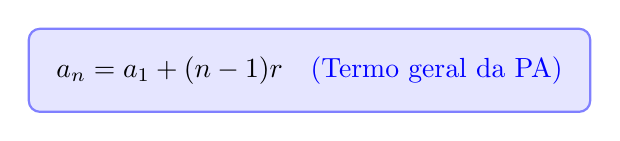
\begin{tikzpicture}
\node[rectangle, fill=blue!10, rounded corners, inner sep=10pt, draw=blue!50, thick] (box) {
$\displaystyle a_n = a_1 + (n-1)r \quad \text{\textcolor{blue}{(Termo geral da PA)}}$
};
\end{tikzpicture}

\vspace{5mm}

\textbf{Onde:}
\begin{itemize}
\item $\textcolor{red}{a_n}$ = termo geral
\item $\textcolor{red}{a_1}$ = primeiro termo
\item $\textcolor{red}{n}$ = posição do termo
\item $\textcolor{red}{r}$ = razão da PA
\end{itemize}

\subsection*{Exemplo}

Calcule a soma quinto termo da PA $(3, 7, 11, 15, \ldots)$
\section*{Soma dos Termos de uma PA}

\subsection*{Fórmula da Soma}

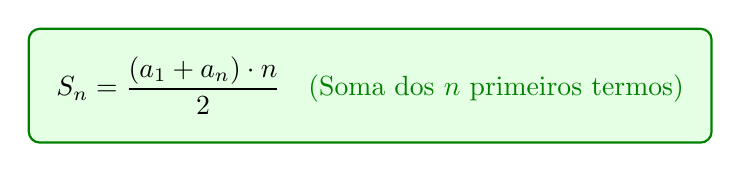
\begin{tikzpicture}
\node[rectangle, fill=green!10, rounded corners, inner sep=10pt, draw=green!50!black, thick] (box) {
$\displaystyle S_n = \frac{(a_1 + a_n) \cdot n}{2} \quad \text{\textcolor{green!50!black}{(Soma dos $n$ primeiros termos)}}$
};
\end{tikzpicture}

\vspace{5mm}

\textbf{Onde:}
\begin{itemize}
\item $\textcolor{blue}{S_n}$ = soma dos $n$ primeiros termos
\item $\textcolor{blue}{a_1}$ = primeiro termo
\item $\textcolor{blue}{a_n}$ = $n$-ésimo termo
\item $\textcolor{blue}{n}$ = número de termos
\end{itemize}

\subsection*{Dedução da Fórmula}

A fórmula pode ser deduzida pelo método de Gauss:
\begin{align*}
S_n &= a_1 + a_2 + a_3 + \cdots + a_n \\
S_n &= a_n + a_{n-1} + a_{n-2} + \cdots + a_1 \\
\hline
2S_n &= (a_1+a_n) + (a_2+a_{n-1}) + \cdots + (a_n+a_1) \\
2S_n &= n \cdot (a_1 + a_n) \quad \text{(pois há $n$ pares iguais)} \\
S_n &= \frac{n(a_1 + a_n)}{2}
\end{align*}

\subsection*{Exemplo}

Calcule a soma dos 20 primeiros termos da PA $(3, 7, 11, 15, \ldots)$

\section*{2. PA como Função Afim Discreta}
Uma PA pode ser vista como uma função afim com domínio nos números naturais:

\[
f: \mathbb{N}^* \rightarrow \mathbb{R}
\]
\[
f(n) = a_1 + (n-1) \cdot r
\]

\section*{Exercícios de Progressão Aritmética (PA)}

\begin{enumerate}[leftmargin=*]

\item Determine o 10º termo da PA $(3, 7, 11, 15, \ldots)$

\item Numa PA, o 5º termo vale 30 e o 9º termo vale 50. Calcule:
\begin{enumerate}[label=\alph*)]
\item A razão da PA
\item O primeiro termo
\item A soma dos 20 primeiros termos
\end{enumerate}

\item Interpole 5 meios aritméticos entre 2 e 14.

\item Calcule a soma dos 25 primeiros termos da PA $(-3, 1, 5, 9, \ldots)$

\item Três números estão em PA. A soma deles é 15 e o produto é 105. Determine esses números.

\item (UFPE) Se a soma dos 15 primeiros termos de uma PA é 150 e o 8º termo é 15, qual é a razão?

\item (ENEM) Um teatro tem 18 filas de cadeiras. Na 1ª fila há 20 cadeiras, na 2ª 23 cadeiras, na 3ª 26, e assim por diante. Quantas cadeiras tem o teatro?

\item Dada a PA $(x-1, 2x, 5x+1)$, determine:
\begin{enumerate}[label=\alph*)]
\item O valor de x
\item A razão da PA
\item O décimo termo
\end{enumerate}

\item Uma escada tem seus degraus construídos de modo que a altura entre degraus consecutivos forma uma PA. Sabendo que o 3º degrau está a 50cm do solo e o 8º a 85cm, calcule:
\begin{enumerate}[label=\alph*)]
\item A altura do 1º degrau
\item A altura do 15º degrau
\end{enumerate}

\item (UERJ) Um ciclista percorre 20km no primeiro dia de treino; no segundo dia, 25km; no terceiro, 30km, e assim sucessivamente. Quantos quilômetros terá percorrido ao final de 30 dias?

\end{enumerate}

\subsection*{Comparação}
    {\footnotesize
\begin{tabular}{|l|l|}
\hline
\textbf{Função Afim Contínua} & \textbf{PA (Função Afim Discreta)} \\
\hline
$f(x) = ax + b$, $x \in \mathbb{R}$ & $f(n) = r \cdot n + (a_1 - r)$, $n \in \mathbb{N}^*$ \\
\hline
Gráfico: reta contínua & Gráfico: pontos alinhados \\
\hline
Taxa de variação constante $a$ & Razão constante $r$ \\
\hline
\end{tabular}
    }

\begin{center}
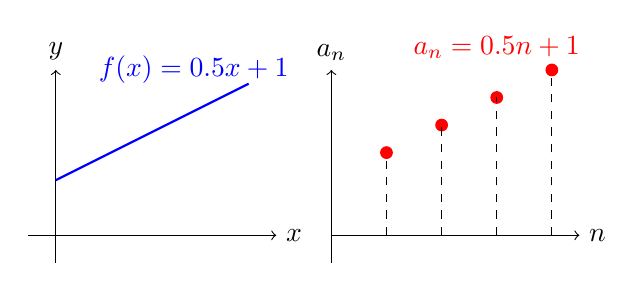
\begin{tikzpicture}[scale=0.7]
% Função afim contínua
\draw[->] (-0.5,0) -- (4,0) node[right]{$x$};
\draw[->] (0,-0.5) -- (0,3) node[above]{$y$};
\draw[blue, thick, domain=0:3.5] plot (\x, {0.5*\x + 1});
\node[blue] at (2.5,3.0) {$f(x)=0.5x+1$};

% PA discreta
\draw[->] (5,0) -- (9.5,0) node[right]{$n$};
\draw[->] (5,-0.5) -- (5,3) node[above]{$a_n$};
\foreach \n in {1,2,3,4} {
    \filldraw[red] (5+\n,{0.5*\n+1}) circle (3pt);
    \draw[dashed] (5+\n,0) -- (5+\n,{0.5*\n+1});
}
\node[red] at (8,3.4) {$a_n=0.5n+1$};
\end{tikzpicture}
\end{center}


\section*{3. Análise de Propriedades}
\subsection*{Taxa de Variação Constante}
Em uma função afim $f(x) = ax + b$, a taxa de variação $\frac{\Delta y}{\Delta x} = a$ é constante.

Na PA:
\[
\frac{a_{n+1} - a_n}{(n+1)-n} = r \quad \text{(constante)}
\]

\subsection*{Linearidade}
Tanto a função afim quanto a PA preservam:
\begin{itemize}
\item Aditividade: $f(n+k) - f(n) = k \cdot r$
\item Homogeneidade: $f(n) - f(1) = (n-1) \cdot r$
\end{itemize}

\section*{4. Aplicação em Problemas}
\subsection*{Exemplo 1}
Uma PA tem $a_5 = 17$ e $a_{10} = 32$. Encontre a função afim correspondente.

\textbf{Solução:}
\begin{align*}
a_5 &= f(5) = 17 \\
a_{10} &= f(10) = 32 \\
\text{Taxa (r)} &= \frac{32-17}{10-5} = 3 \\
a_1 &= 17 - (5-1)\cdot3 = 5 \\
\text{Função: } & f(n) = 3n + 2
\end{align*}

\subsection*{Exemplo 2}
Uma escada tem degraus onde a altura entre eles segue uma PA. O 3° degrau está a 42cm do chão e o 7° a 78cm. Qual a altura do 1° degrau?

\textbf{Solução:}
Modelando como função afim discreta:
\begin{align*}
f(3) &= 42 \\
f(7) &= 78 \\
r &= \frac{78-42}{7-3} = 9 \\
f(1) &= 42 - (3-1)\cdot9 = 24 \text{ cm}
\end{align*}

\section*{5. Exercícios}
\begin{enumerate}
\item Associe cada PA à sua função afim correspondente:
\begin{enumerate}[label=\alph*)]
\item $2, 5, 8, 11, \ldots$ \quad ( ) $f(n) = 4n - 1$
\item $3, 7, 11, 15, \ldots$ \quad ( ) $f(n) = 3n - 1$
\item $-1, 3, 7, 11, \ldots$ \quad ( ) $f(n) = 4n - 5$
\end{enumerate}

\item Dada a PA com $f(3) = 10$ e $f(7) = 26$, determine:
\begin{enumerate}[label=\alph*)]
\item A razão $r$
\item O termo inicial $a_1$
\item A expressão da função afim $f(n)$
\end{enumerate}

\item Um serviço de entregas cobra R\$ 5,00 fixos mais R\$ 2,00 por km. Modele como:
\begin{enumerate}[label=\alph*)]
\item Função afim contínua
\item PA discreta (para km inteiros)
\item Calcule o custo para 15 km em ambos modelos
\end{enumerate}

\end{enumerate}

\end{multicols}

\end{document}
